\selectlanguage{italian}%

\section{Soluzione}


\subsection{Schematico}

\subsubsection{GPIO}

\begin{figure}[H]
	\centering
	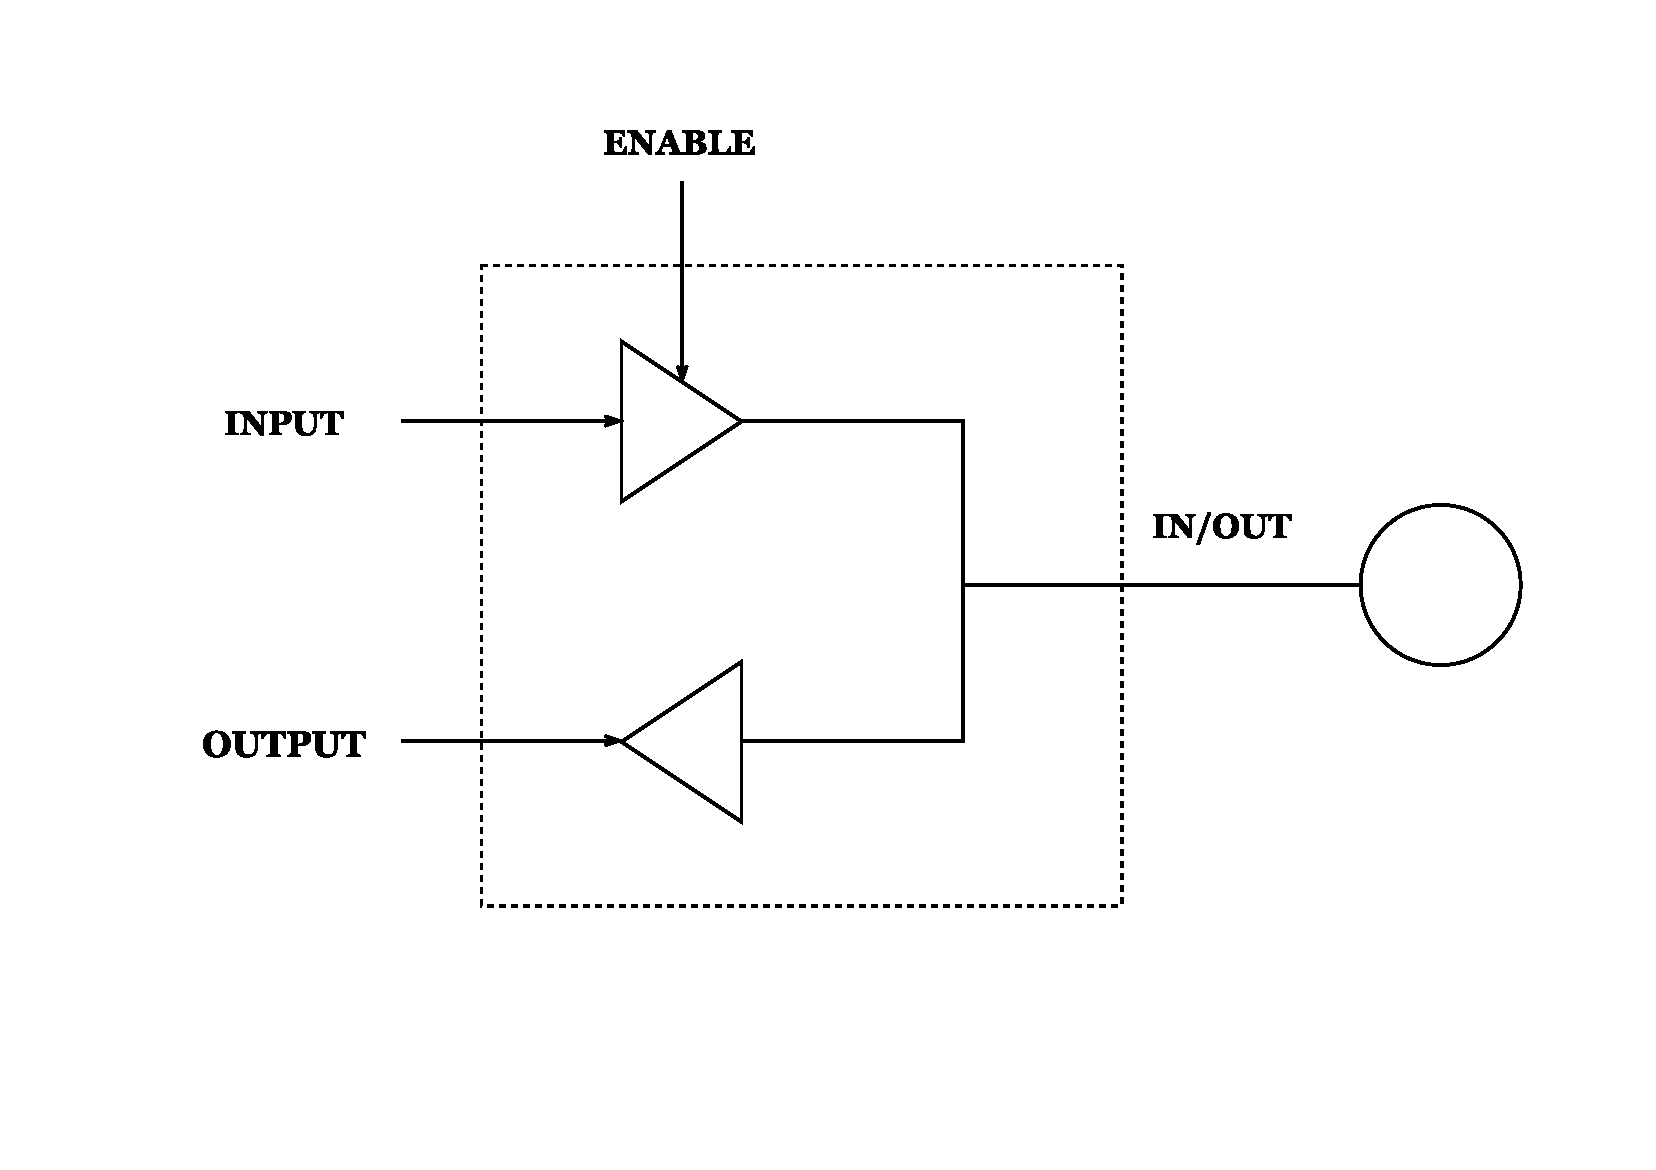
\includegraphics[scale=0.7]{esercizio16/images/GPIO.png}
	\caption{GPIO Schematic}
	\label{fig:GPIO_schematics}
\end{figure}

\subsection{Codice}

Progetto ISE: \href{run:progetti/GPIO/GPIO.xise}{GPIO ISE}


\subsubsection{Pad}

Questo componente, rappresentato in Figura \ref{fig:GPIO_schematics}
decide se l'operazione da effettuare � di scrittura o di lettura in
base al valore del segnale di enable. Quando enable � alto, si effettua
una scrittura e il segnale di input/output \textit{in\_out }viene
caricato con il valore del segnale di input, poi trasferito al segnale
di output. Quando enable � basso si effettua un'operazione di lettura
quindi, per evitare di disturbare il valore da leggere, viene spento
il buffer, ponendo il segnale in\_out ad alta impedenza ('Z'). Questo
comportamento � modellato tramite un costrutto dataflow \textit{with-select.}\\
Il componente in questione � osservabile a questo link: \href{run:progetti/GPIO/pad.vhd}{Pad}

\subsubsection{GPIO}

Questa � una top-level entity che si preoccupa di creare, tramite
un \textit{for-generate, }una serie di pad, il cui numero � settato
tramite un generic. \\
Il componente in questione � osservabile a questo link: \href{run:progetti/GPIO/gpio.vhd}{GPIO}\selectlanguage{italian}%

